%!TEX root = ../main_wo_rep.tex
%
% 電流と磁場
%


\section{電流と磁場}

\subsection{電流が磁場から受ける力と電流が作る磁場}

\begin{wrapfigure}[6]{r}{6cm}
\vspace*{-0.4cm}
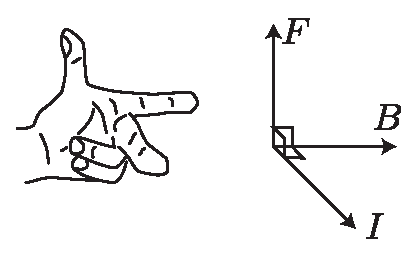
\includegraphics[scale=0.9]{07_EleMag/FBI.eps}
\end{wrapfigure}


動いている電荷(=電流)は磁場から力を受けることが知られています。点電荷$q$が磁
束密度$B$から受ける力は、点電荷が磁場の向きに対して垂直な向きに速度$v$で
動いているとすると、$F=qvB$の大きさの力を受けます。この力を{\bf ローレンツ力}といい、
力を受ける向きは、{\bf フレミングの左手の法則}によって表されます。(電流$I$の向きは、負
の電荷を持つ電子の進む方向とは逆向きなので注意しましょう。)

また、動いている電荷(電流)自身が周囲に磁場を作ることも知られています。電流が
作る磁場の強さを表す法則は、{\bf ビオ・サバールの法則}と呼ばれています。

\subsection{電磁誘導(磁場が作る電流)}

1831年にファラデーは、コイルに磁石を近づけたり遠ざけたりすると、コイルに電
流が流れること発見しました。この現象を{\bf 電磁誘導}といいます。

この現象は、コイルを固定して磁石を動かす代わりに磁場の中でコイルを動かして
も起こり、コイルや回路の中を垂直に貫く磁場の強さが時間的変化をすると、磁場の強
さがどの程度変化するかに応じて流れる電流の量が変わります。

この原理を利用したものには、発電機、変圧器、マイク(ダイナミックマイク)などがあります。


\bigskip

\begin{itembox}[l]{\bf コラム:交流モーターの話}
皆さんが本授業で作るモーターは乾電池で動くもので、直流モーターです。交流電源
に接続しても動きません。このモーターに使われているネオジム磁石を電磁石に置き換
えて電機子と直列に接続すると直流直巻モーターになります。ところが、この種のモーター
は交流でも動くので、一般にユニバーサルモーターと呼ばれていて、扇風機や電気掃除
機等に利用されています。但し、音がうるさいという難点があります。

{\bf 注意:} 皆さんが作成する簡易モーターをユニバーサルモーターに改造してコンセント 
(100ボルトの交流電源)につながないこと。非常に危険です!
\end{itembox}



\newpage

\jikken

\begin{itemsquarebox}[c]{\bf 実験用具}
エナメル線、みの虫クリップの導線2本、単一乾電池、ネオジム磁石、
セロテープ、紙、紙コップ、紙やすり、カッターマット、ミニアンプ、ノートパソコン、
単三乾電池、ブレッドボード、ゼムクリップ(小) 2個、ニッパー
\end{itemsquarebox}

\bigskip

\subjikken{簡易スピーカーの作成}

\begin{enumerate}

\item まず、エナメル線を3 mほど切り取り、単一乾電池に巻きつけてコイルを作ります。コイルの巻
き数は$30\sim 50$回ほどにし、コイルの端はそれぞれ15 cmほどエナメル線を出して
切断しておきます。コイルはケースからはずし、ばらばらにならないように2ケ
所程度をセロテープで軽くとめておきます。

\item 紙コップの底の裏に、コイルをセロテープで貼り付けます。(2ヶ所をとめればよ 
い。)

\item 次に、磁石を別の紙に貼り付け、磁石がコイルの中に入るように注意して、その
紙をコップの裏に貼り付けます。

\item コイルの両端のエナメル線の被膜を、紙やすりではがし、
コイルの両端をミニアンプのスピーカー端子に接続します。

※ 紙やすりで被膜をはがすときは実験机を傷つけないよう、必ずカッターマットの上で作業しましょう。


\item ミニアンプの入力をノートパソコンのイヤホン出力と接続し、
ノートパソコンで音楽を再生します。音量をあげて紙コップを耳に当て、
音が聞こえてくるか、確かめましょう。

\item 磁石の種類を変えたり、ハガキや厚紙などの紙や、紙以外の材質(プラスチック
など)でも試してみて、音が大きくきれいに出せる条件を考えてみましょう。

\item 作成したスピーカーのエナメル線をオシロスコープのCH1に接続し、スピーカーに向かって
声を出してオシロスコープの表示を観察しましょう。
オシロスコープに声の波形が表示されることからスピーカーが
マイクとして作用していることがわかりますが、なぜマイクとして
働くのかについても考えてみましょう。

%\hspace*{-\parindent}
%※ なぜ音が聞こえるのか、考察しましょう。また、まったく同じ仕組みでマイクが
%作れますが、なぜマイクとして働くのかについても考察しましょう。


\end{enumerate}



\newpage

\subjikken{簡易モーターの作成}

\begin{enumerate}

\item エナメル線を50 cmほど切り取り、
エナメル線の端を5 cm程度残して、{\bf 単三乾電池}に10回ほど巻きつけてコイルを
作ります。コイルは巻き始めと巻き終わりの左右の2箇所にエナメル線を巻きつ
けて固定しておきます(2回ほど巻いておけば良い)。下の図のような形になりま
すが、このとき左右のエナメル線がちょうどコイルの中心の高さを通るように気
をつけて作成します。
\begin{center}
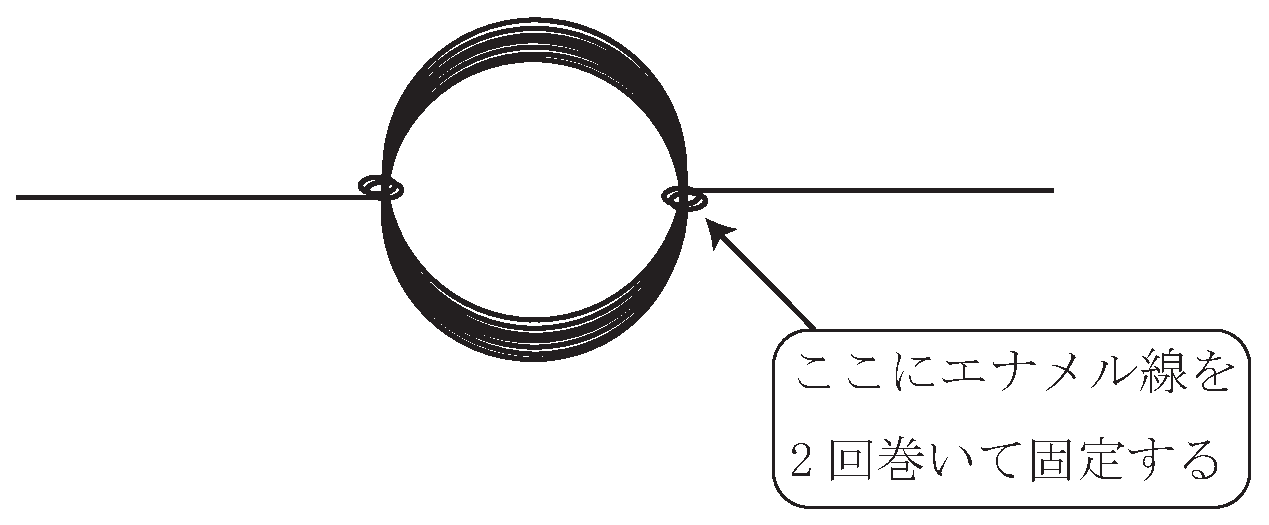
\includegraphics[scale=0.45]{07_EleMag/coil.eps}
\end{center}

\item
\begin{minipage}[t]{10cm}
クリップ2個の先を図のように伸ばし、10$\sim$15個ほどの穴の間隔
をあけて土台にするブレッドボードの穴に刺しておきます。
\end{minipage}
\begin{minipage}[c]{3cm}
\hspace*{1cm}
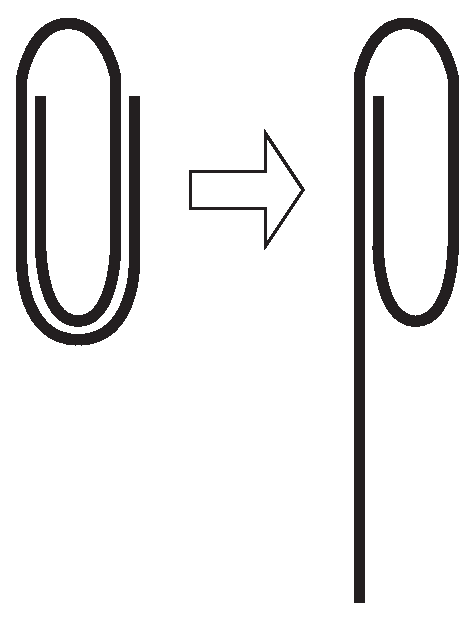
\includegraphics[scale=0.35]{07_EleMag/clip.eps}
\end{minipage}

\item コイルから出ているエナメル線の長さを適当な長さ
(1.5 cm$\sim$2 cm)に切り、先端の1 cmほどを、片方は紙
やすりを使って被膜を全部剥がし、もう一方は半分のみ
剥がしておきます。

※ 紙やすりで被膜をはがすときは実験机を傷つけないよう、必ずカッターマットの上で作業しましょう。


\item ブレッドボードに刺したクリップに通電するように導線をつなぎます。
(ブレッドボードの穴どうしは列単位で電気的に接続されています。)
さらに、クリップとクリップの真ん中に来るように、
ネオジウム磁石をブレッドボードにセロテープでとめておきます。

\item 2本のクリップを軸受けにしてコイルを設置し、ブレッドボードからの導線の
端を乾電池につなぎ、コイルを軽く指で押して回転させてやります。(回転の向き
に注意すること。)

\hspace*{-\parindent}
※ うまくできていれば、そのままコイルは勢い良く回転し続けます。

\item オシロスコープを使ってモーターのコイルにかかる電圧の変化を
観察してみましょう。電圧の変化からどのようなことがわかるでしょうか?

\end{enumerate}

